In this chapter we will give a brief introduction of Machine Learning (\ref{ml}), explaining Classification (\ref{classification}), Regression (\ref{regression}), Supervised (\ref{supervised}) and Unsupervised (\ref{unsupervised}) Learning, proceding then to explain SVM (\ref{svm}) which is the most important technique used for this thesis.

\section{Machine Learning} \label{ml}
Machine Learning is a subfield of Artificial Intelligence that uses statistical techniques to provide computers with the ability to progressively improve performance on different tasks using data, while not being explicitly programmed \cite{wiki:ml}. \\
The application for machine learning are huge and diverse, and range from character recognition to email filtering, with lots of application in computer vision, such as image recognition and classification. \\
Machine learning also focuses on making prediction on data, by utilizing techniques taken from mathematical optimization. This has many applications, ranging from health care by predicting risk factors for diseases or gaining insights for prevention, to sports or politics where actual results can be predicted.\\
The field of machine learning is subdivided in two broad categories (Fig. \ref{fig:ml_mldiv}), supervised learning (\ref{supervised}) and unsupervised learning (Fig. \ref{unsupervised}) based on whether the data is labeled or not.\\

\begin{figure}[H]
	\centering
	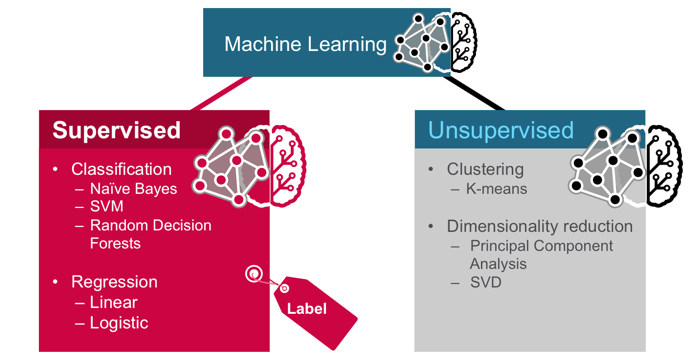
\includegraphics[width=0.5\textwidth]{ml_mldiv}
	\caption{Machine Learning Subfields \cite{ml_mldiv}}
	\label{fig:ml_mldiv}
\end{figure}

Another classification is based on the kind of output that the users wish to obtain, mainly Classification (\ref{classification}), Regression (\ref{regression}) or Clustering.

% TODO: Section or SubSection?
\subsection{Supervised Learning} \label{supervised}
When using supervised learning we want to learn a function that maps an input to an output, based on example input-output pairs \cite{ai_sup}. This means that we need labeled training data, consisting of a vector of input objects and an output value. The objective is to correctly classify the new data based on the analyzed training pairs. \\
The general steps to solve a supervised learning problem are (Fig. \ref{fig:sup_wf}):
\begin{enumerate}
	\setlength{\itemsep}{0pt}
	\item Understand what kind of training example to use.
	\item Gathering a training set.
	\item Model the training set to be fed as input to the algorithm by choosing which features to use and how to represent the data.
	\item Choose what kind of algorithm can best train the model.
	\item Run the algorithm and evaluate the resulting accuracy on the test set 
\end{enumerate}

\begin{figure}[H]
	\centering
	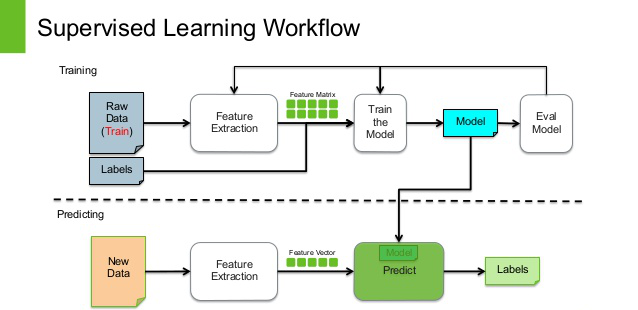
\includegraphics[width=0.5\textwidth]{sup_wf}
	\caption{Supervised Learning Workflow \cite{sup_wf}}
	\label{fig:sup_wf}
\end{figure}

There are important considerations to make when using a supervised learning approach:
\begin{itemize}
	% TODO: Write this better
	\item \textbf{Bias-Variance Tradeoff} \cite{biasvar}: suppose we have different (but equally good) training set. An algorithm is biased for input x if, when trained on each of these data sets, it is consistently incorrect at predicting the correct output for x. \\
	A learning algorithm has high variance for a particular input x if it predicts different output values when trained on different training sets. \\
	The prediction error of a classifier is related to the sum of bias and variance, so generally there is a tradeoff between them. Low bias means that it fits the new data well, but if the bias is too low it will fit each training set differently and so result in high variance.
\end{itemize}

\subsection{Unsupervised Learning} \label{unsupervised}

\subsection{Classification} \label{classification}

\subsection{Regression} \label{regression}

\pagebreak

\section{SVM} \label{svm}
Support Vector Machines (SVM) are a supervised machine learning algorithm used for both classification and regression. \\
The main idea is to find the optimal hyperplane for linearly separable data, and then extend this idea to data that are not linearly separable by mapping this data in a new space using a kernel function.\\
The definition of an hyperplane for p-dimensions is:
\begin{equation}
\beta_0 + \beta_1 X_1 + \beta_2 X_2 + \dots + \beta_p X_p = 0
\end{equation}

Support vectors are the data points that lie closest to the hyperplane (Fig. \ref{fig:suppvec}), they also are the data points most difficult to classify and have direct bearing on the optimum location of the hyperplane.\\
\begin{figure}[h]
	\centering
	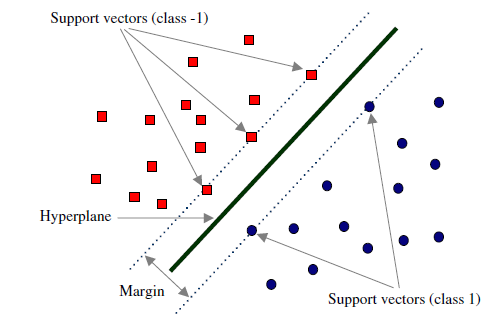
\includegraphics[width=0.5\textwidth]{svm_support_vectors}
	\caption{Example of Support Vectors}
	\label{fig:suppvec}
\end{figure}

The distance between the hyperplane and the nearest data point from either set is known as the margin. The best hyperplane is the one that maximizes the margins for the data we are classifying.\\
\begin{figure}[H]
	\centering
	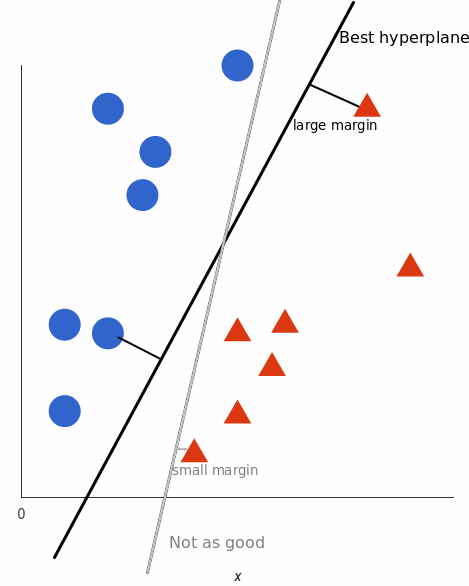
\includegraphics[width=0.5\textwidth]{hyperplane_margin}
	\caption{Different hyperplanes with different margins \cite{svm_monkeylearn}}
\end{figure}

So the objective is to choose a hyperplane with the largest possible margin between it and the support vectors, since the larger is the margin, the lower the generalization error of the classifier.\\
In essence, support vectors are the elements of the training set that would change the position of the dividing hyperplane if removed. This makes the support vectors the critical elements of the training set.\\

Finding the maximal margin hyperplane based on a set of training observations $x_1, \dots x_n \in R^p$ and with class lables $y_1 \dots y_n$, translates to an optimization problem:

Maximize M
\begin{equation}
\beta_0, \beta_1, \beta_2, \dots, \beta_p, M
\end{equation}

subject to
\begin{equation}
\sum_{j=1}^{p}\beta^2_j = 1
\end{equation}

\begin{equation}
y_i(\beta_0 + \beta_1 X_i1 + \beta_2 X_i2 + \dots + \beta_p X_ip) \ge M \forall i = 1, \dots, n
\end{equation}

2.3 and 2.4 ensure that each observation is on the correct side of the hyperplane and at least a distance M from the hyperplane. Hence, M represents the margin of our hyperplane, and the optimization problem chooses $\beta_0, \beta_1, \beta_2, \dots, \beta_p$ to maximize M. \\
Unfortunately this hyperplane does not necessarily exists, but we can extend this concept to find a hyperplane that almost separates the classes using a soft margin. This is what an SVM does.

It is very probable that the data is not linearly separable, as we can see in figure \ref{fig:svmnotsep}.
\begin{figure}[H]
	\centering
	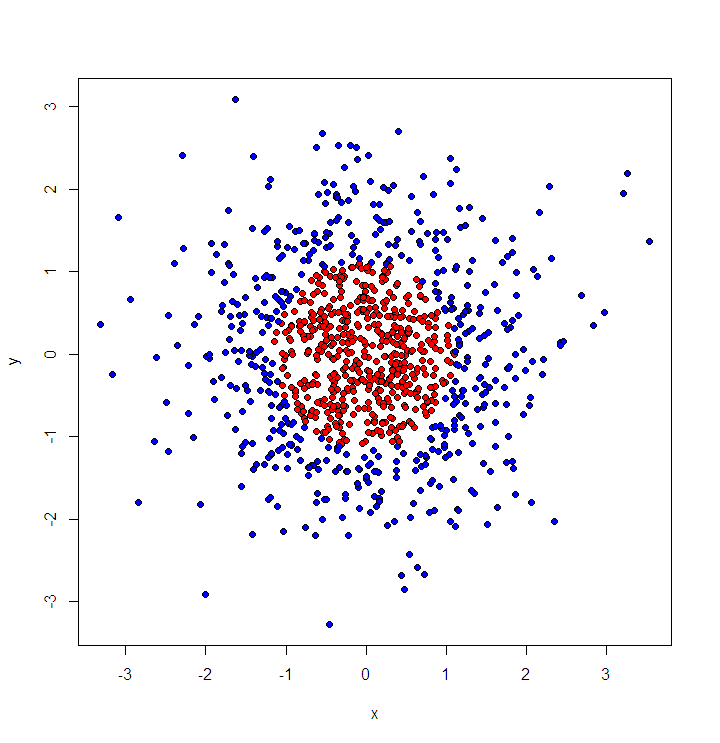
\includegraphics[width=0.5\textwidth]{svm_not_separable}
	\caption{Linearly not separable data \cite{svm_monkeylearn}}
	\label{fig:svmnotsep}
\end{figure}

In this case, for example, we can add a new dimension and separate the data. 
\begin{figure}[H]
	\centering
	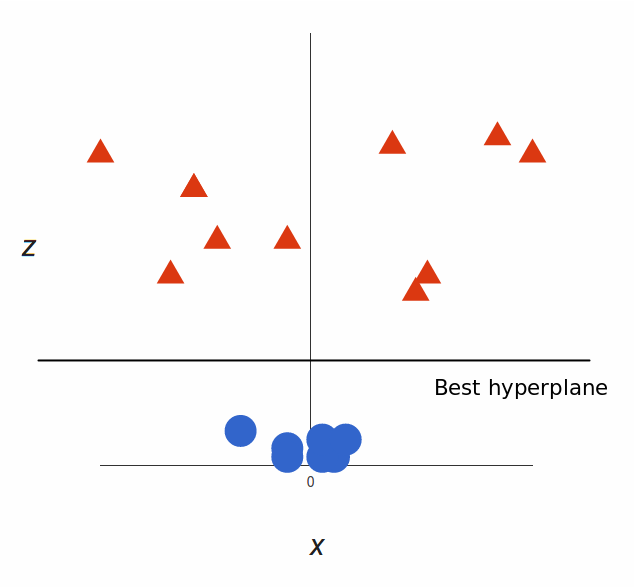
\includegraphics[width=0.5\textwidth]{svm_three_dim}
	\caption{Three dimensional separable space \cite{svm_monkeylearn}}
\end{figure} 

And then map back to two dimension.
\begin{figure}[H]
	\centering
	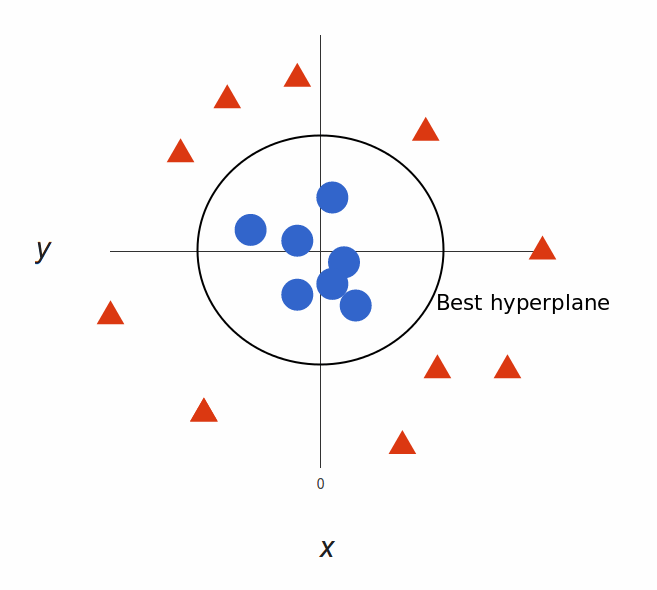
\includegraphics[width=0.5\textwidth]{svm_separated}
	\caption{Separated data \cite{svm_monkeylearn}}
\end{figure}



Calculating the transformation can be very computationally intensive, but SVM just needs the dot product between the vectors. This is called the kernel function. Kernels can be of different types, like linear or 
